\subsection{Evaluation}
\label{norax:sec:eval}
We evaluate three aspects of \norax: (i) whether it breaks the functioning of patched binaries? (ii) how accurate is its data analysis? and (iii) how much overhead it incurs?

\point{Functioning of Transformed Binaries} 
For this test, we selected 20 core system binaries to transform, including both programs and
libraries (Table~\ref{tab:eval-rewrite}).  These binaries provide support for
basic functionalities of an Android phone, such as making a phone call,
installing apps, and playing videos.  We obtain these binaries from a
Nexus 5X phone that runs Android OS v6.0.1 (Marshmallow). These stock
binaries are compiled with compiler optimization and without debugging metadata. 

We tested the functionality of the transformed binaries using our
own test cases as well as the Android Compatibility Test Suite
(CTS)~\cite{cts}. We modified the system bootstrapping
scripts (\emph{$*.rc$} files), which direct Android to load the system binaries patched by \NORAX. 
%run the retrofitted executables with
%the rewritten libraries using the LD\_PRELOAD environment variable. 
Table~\ref{tab:eval-intro} shows the specific tests we designed for
each system executable and library. 
For example,  $surfaceflinger$ is the UI composer, which depends on two libraries:
$libmedia.so$ and $libstagefright.so$. 
Zygote ($app\_process\textit{64}$) is the template process from which all App processes 
are forked. It uses all of the patched binaries.  
While running our functionality tests, we observed an attempt by the
linker to read the ELF header, which is located in the pages
marked executable-only. While this attempt was allowed and facilitated by \NMonitor, our system can
be optimized to handle this case during the patching stage instead. 

We also ran the Android Compatibility Test Suite (CTS) on a system
where our transformed binaries are installed.  The suite contains around 127,000
test packages, and is mandatory test  performed by OEM vendors to assess the compatibility
of their modified Android systems. The test results are shown in Table~\ref{tab:cts}. 
\NORAX did not introduce any additional failure than those generated by the vendor customization on the testing devices. The results from both tests show that the functioning of patched binaries is not interrupted or broken by \NORAX. 

\point{Correctness of Data Analysis}
To thoroughly test the correctness of our embedded data identification algorithm, we ran the data analysis module of \NDisassembler against a large test set consisting of all 313 Android system binaries, whose sizes span from 5.6KB (\textit{libjnigraphics.so}) to 16.5MB (\textit{liblog.so}), totaling 102MB. 
For these binaries, we compare the data identified by \textit{\NDisassembler} with the real embedded data. Our ground truth is obtained by compiling debugging sections (.debug\_*)\cite{dwarf} into the binaries. We use an automatic script to collect bytes in file offsets that fall outside any function range and compare them with the analysis results from \textit{\NDisassembler}. For the bytes that are not used by any of the functions, we found that some of them are {\it{NOP}} instructions used purely for the padding purpose; whilst some are just ``easter eggs'', for instance, in the function \textit{gcm\_ghash\_v8} of \textit{libcrypto.so}, the developers left a string \textit{``GHASH for ARMv8, CRYPTOGAMS by $<$appro@openssl.org$>$''}. These kinds of data were not collected by \NORAX. Since there are no references to them, making them non-readable will not break any function. 

For the tested binaries, \textit{\NDisassembler} correctly identified all the embedded data.  Only for 28 out of the 313 binaries did \NDisassembler reported false positives (i.e., code mistakenly identified as embedded data), due to the over-approximate approach we use. These rare false positive cases are expected by our design and are handled by \NMonitor during runtime. 
Table~\ref{tab:embedgadgets} shows a subset of the results\footnote{This subset was chosen to be consistent with the binaries used in the other tests in this section. The complete set of all 313 Android system binaries, which can be easily obtained, are not shown here due to the space limit.}.

%--rewrite outcome correctness, 
\begin{table*}[h]
	\centering
	\begin{minipage}[b]{0.45\textwidth}
		\centering	
		\caption{Rewritten program functionality tests.}
		\label{tab:eval-intro}
		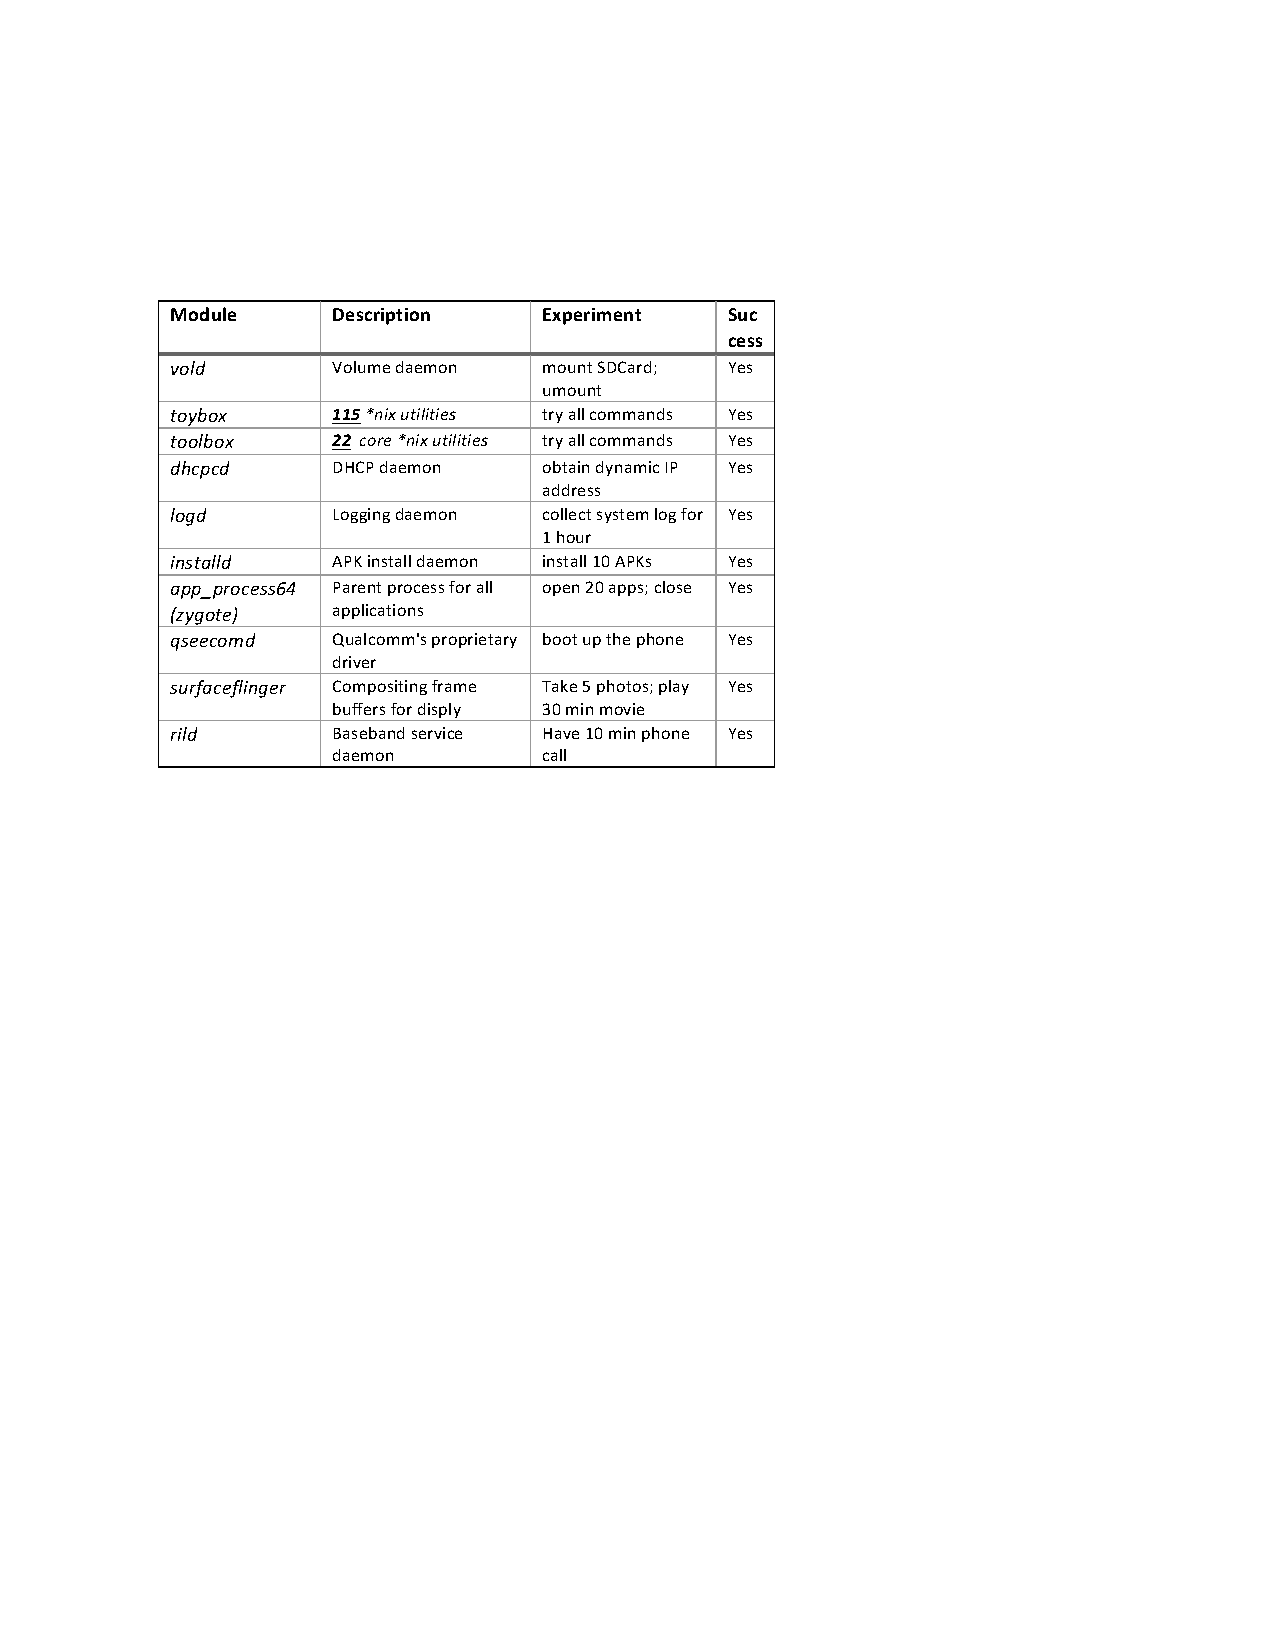
\includegraphics[scale=0.76]{norax/figures/realworld-task}
	\end{minipage}
 	\hfill
	\begin{minipage}[b]{0.5\textwidth}
		\centering	
		\caption{System compatibility evaluation, the converted zygote, qseecomd, installd, rild, logd, surfaceflinger, libc++, libstagefright are selected randomly to participate the test to see whether they can run transparently with other unmodified system components.}
		\label{tab:cts}
		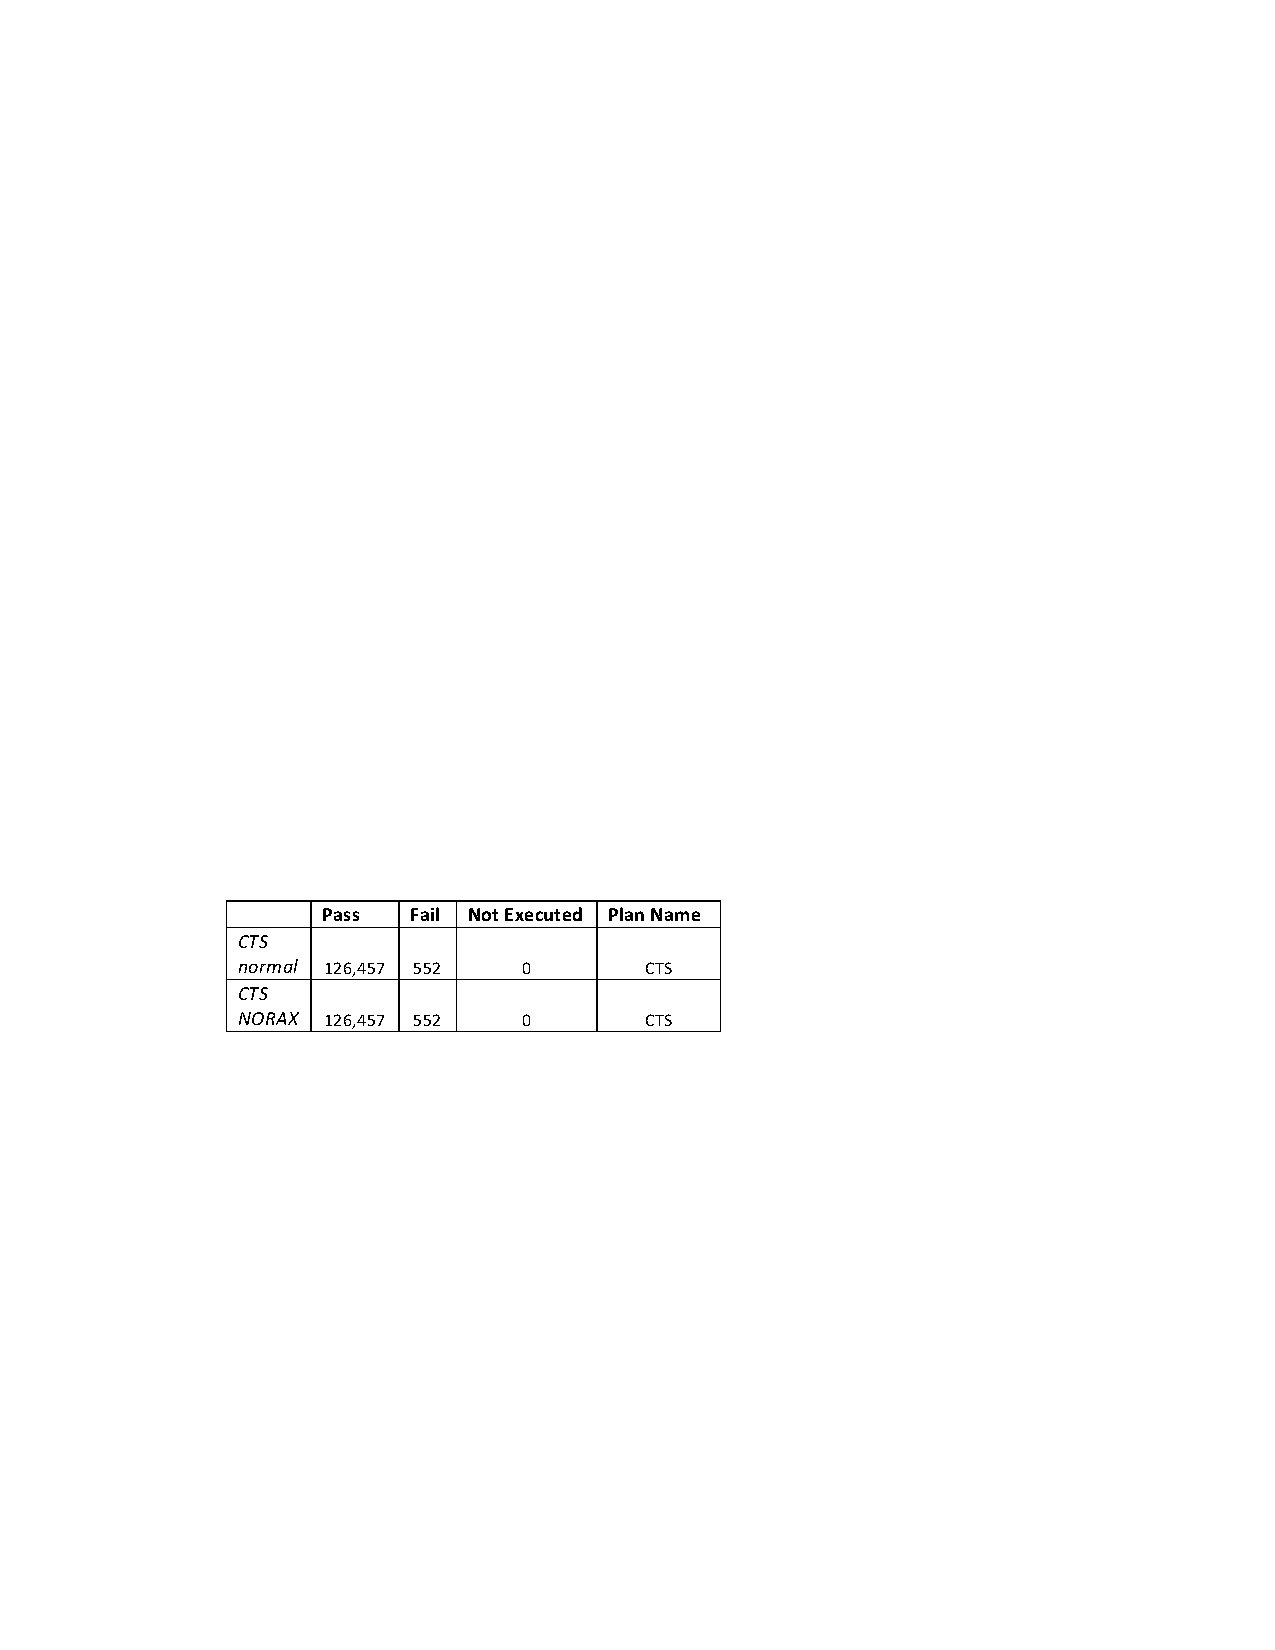
\includegraphics[scale=0.80]{norax/figures/cts}
	\end{minipage}
\end{table*}




%
%\begin{table}[ht]
%\caption{Rewritten program functionality tests.}
%\label{tab:eval-intro}
%\begin{center}
%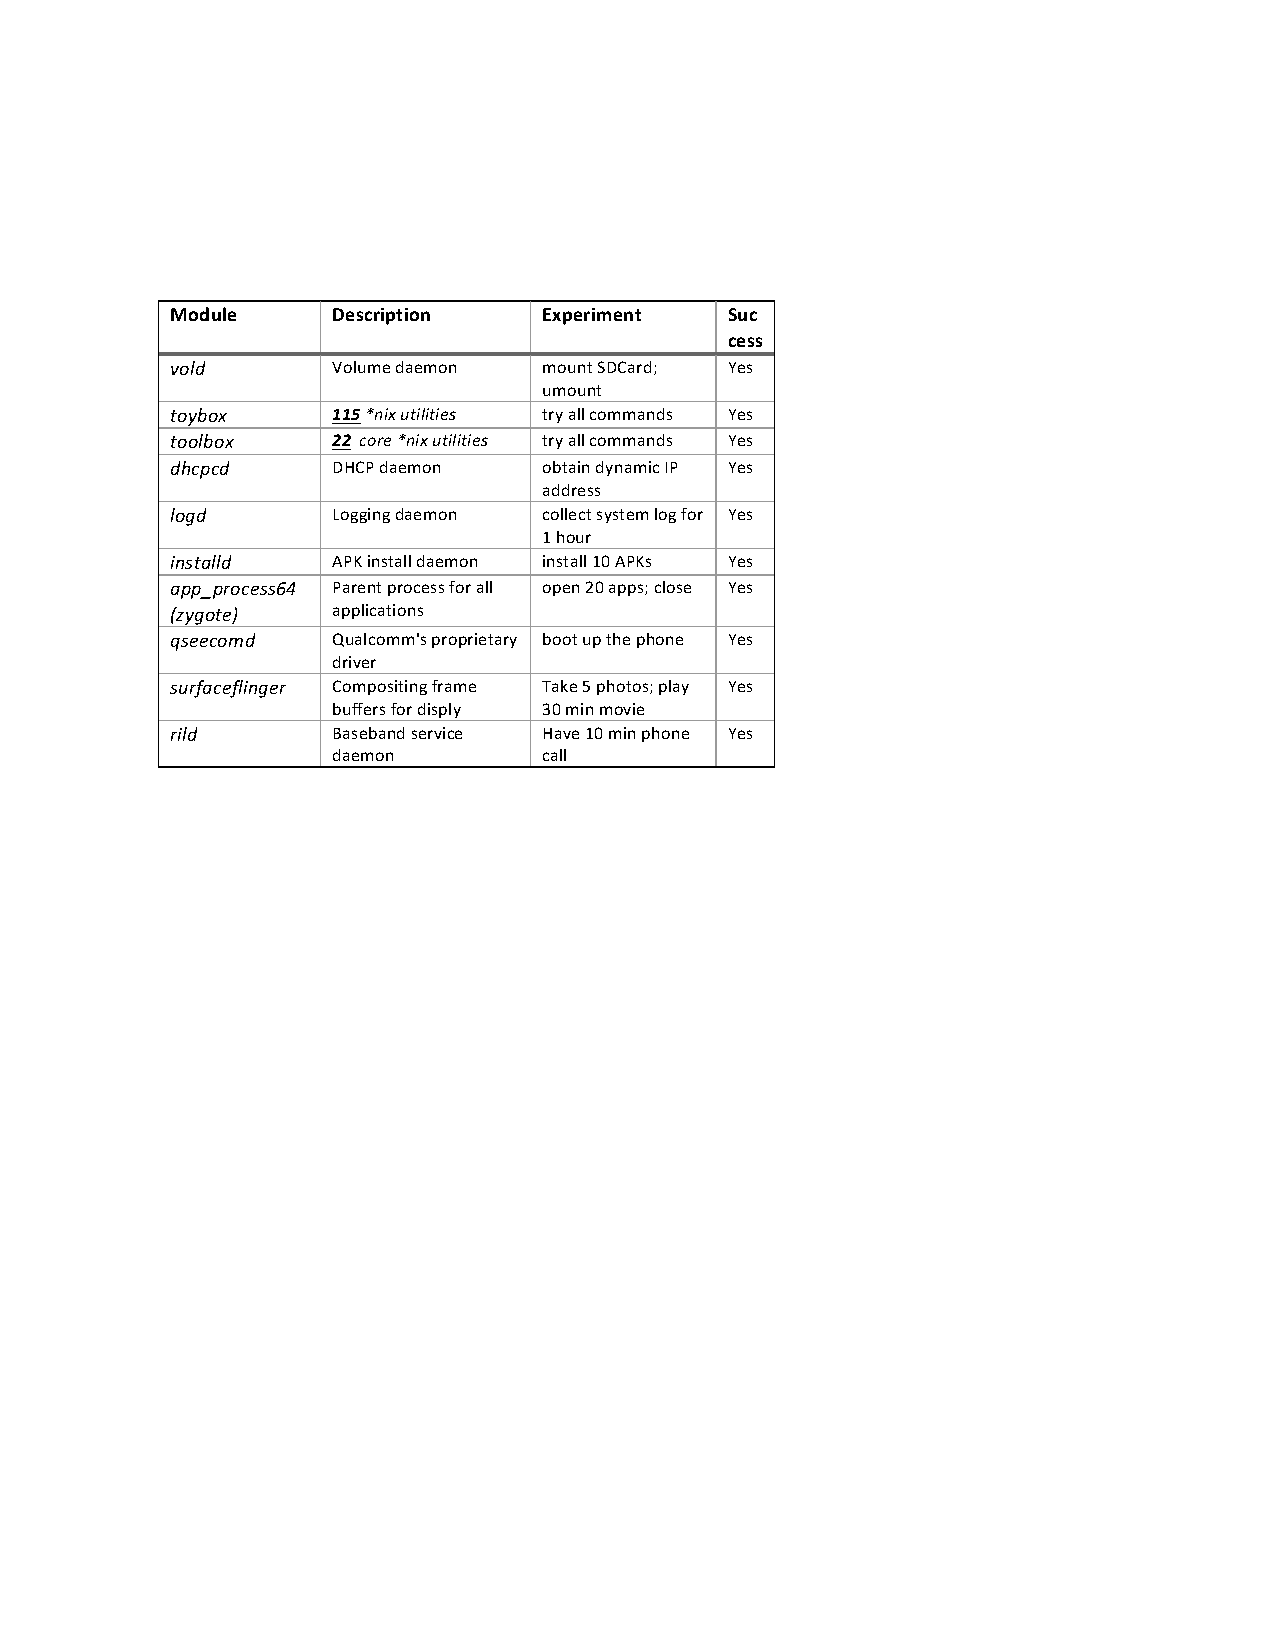
\includegraphics[scale=0.76]{norax/figures/realworld-task}
%\end{center}
%\end{table}
%
%%--comprehensive compatibility evaluation
%\begin{table}[ht]
%\caption{System compatibility evaluation, the converted zygote, qseecomd, installd, rild, logd, surfaceflinger, libc++, libstagefright are selected randomly to participate the test to see whether they can run transparently with other unmodified system components.}
%\label{tab:cts}
%\begin{center}
%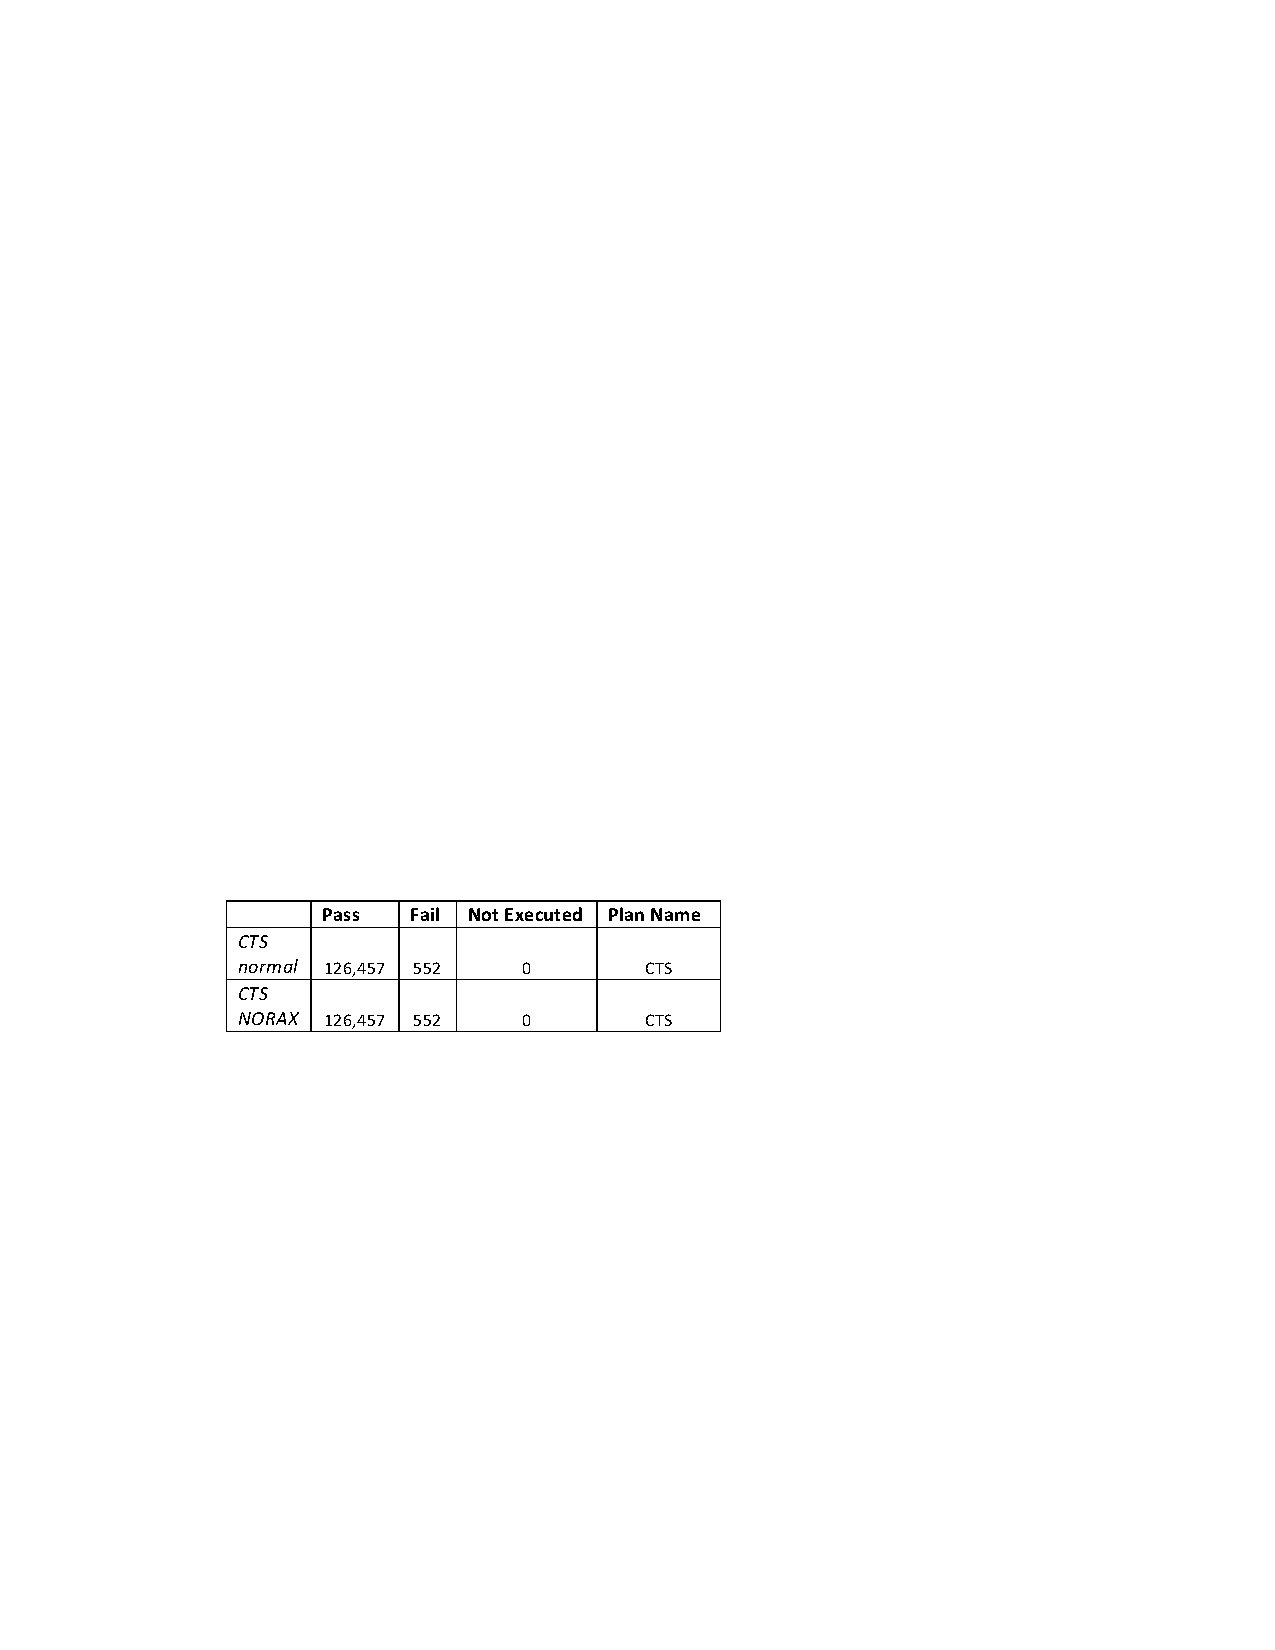
\includegraphics[scale=0.80]{norax/figures/cts}
%\end{center}
%\end{table}

%--rewrite correctness, 

\begin{table*}[h]
	\centering
	\begin{minipage}[b]{0.45\textwidth}
		\centering	
\caption{Binary transformation correctness test.}
\label{tab:eval-rewrite}
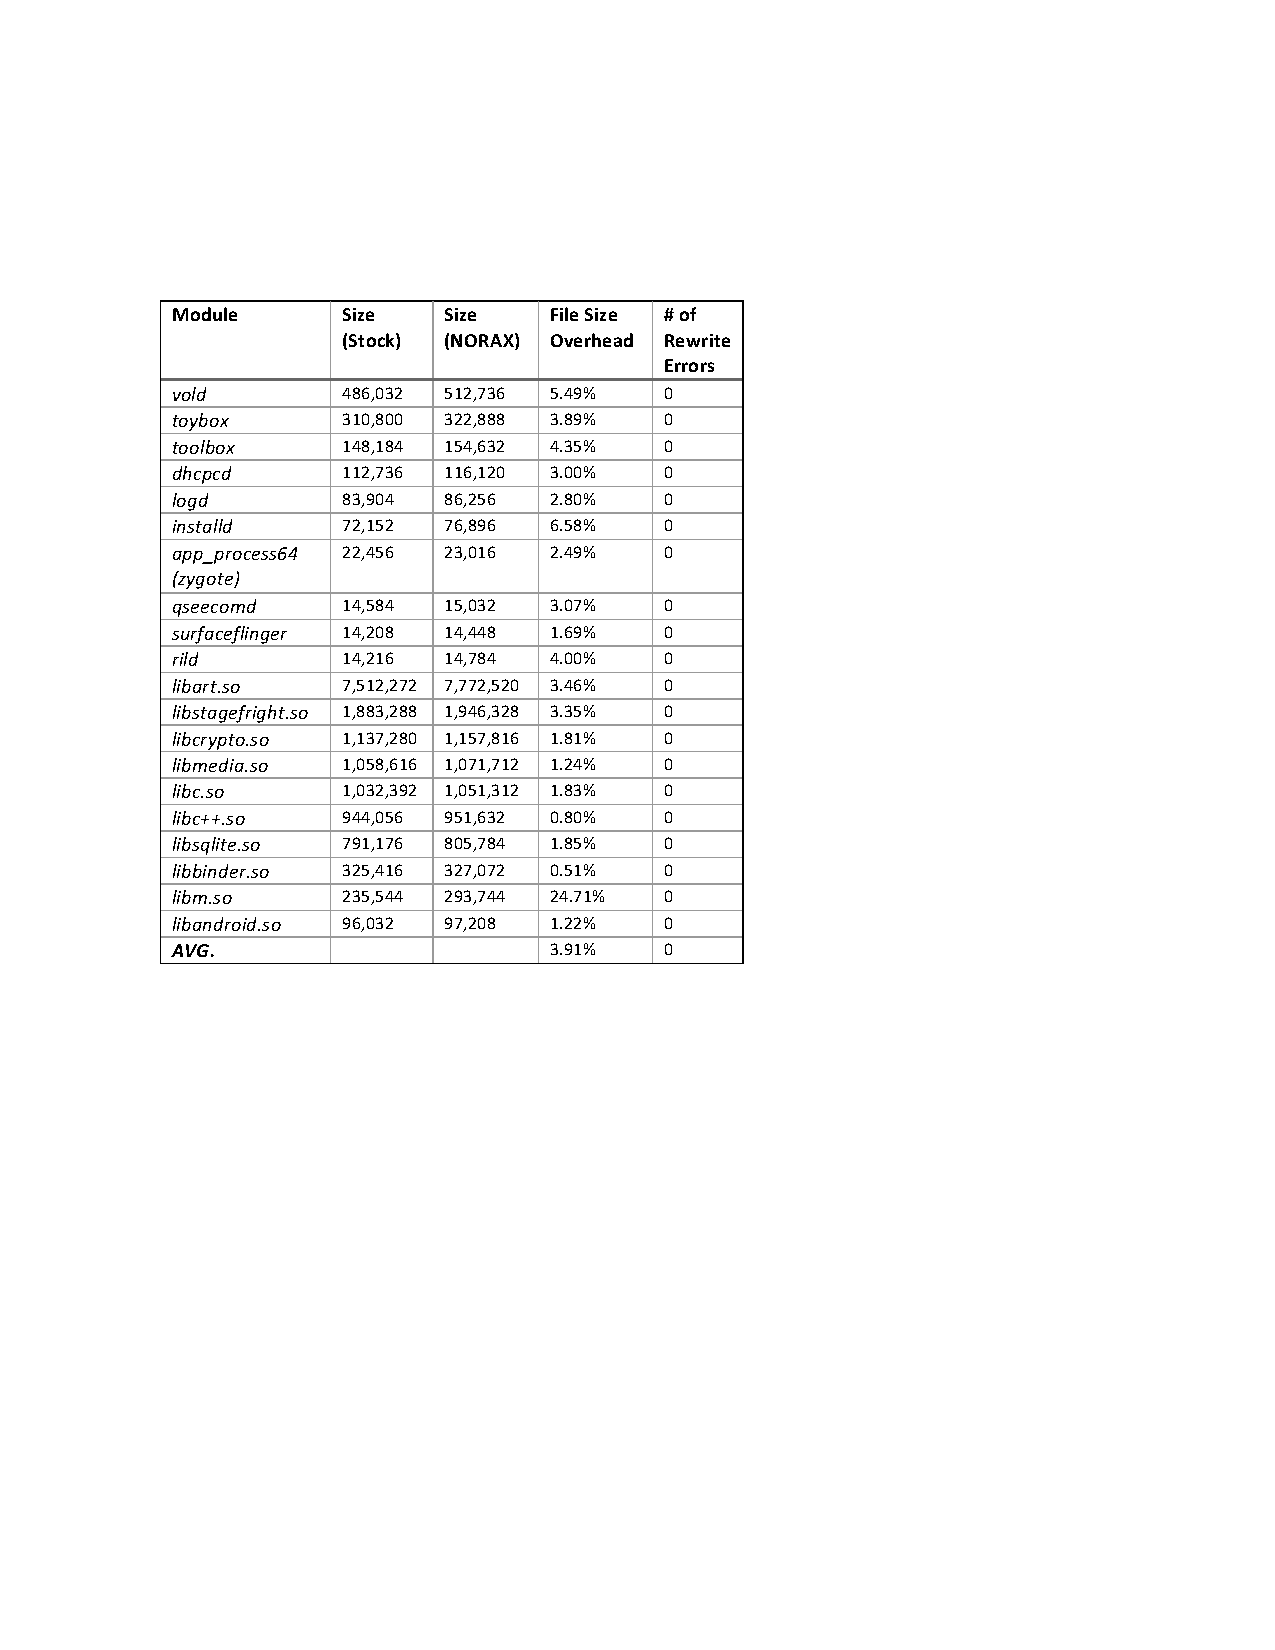
\includegraphics[scale=0.80]{norax/figures/rewrite-correctness}
	\end{minipage}
 	\hfill
	\begin{minipage}[b]{0.5\textwidth}
		\centering	
\caption{Embedded data identification correctness, empirical experiment
shows our analysis works well in AArch64 COTS ELFs, with {\bf zero} false negative rate and very low false positive rate in terms of finding embedded data. The last column shows the negligible number of leftover gadgets in the duplicated embedded data set.}
\label{tab:embedgadgets}
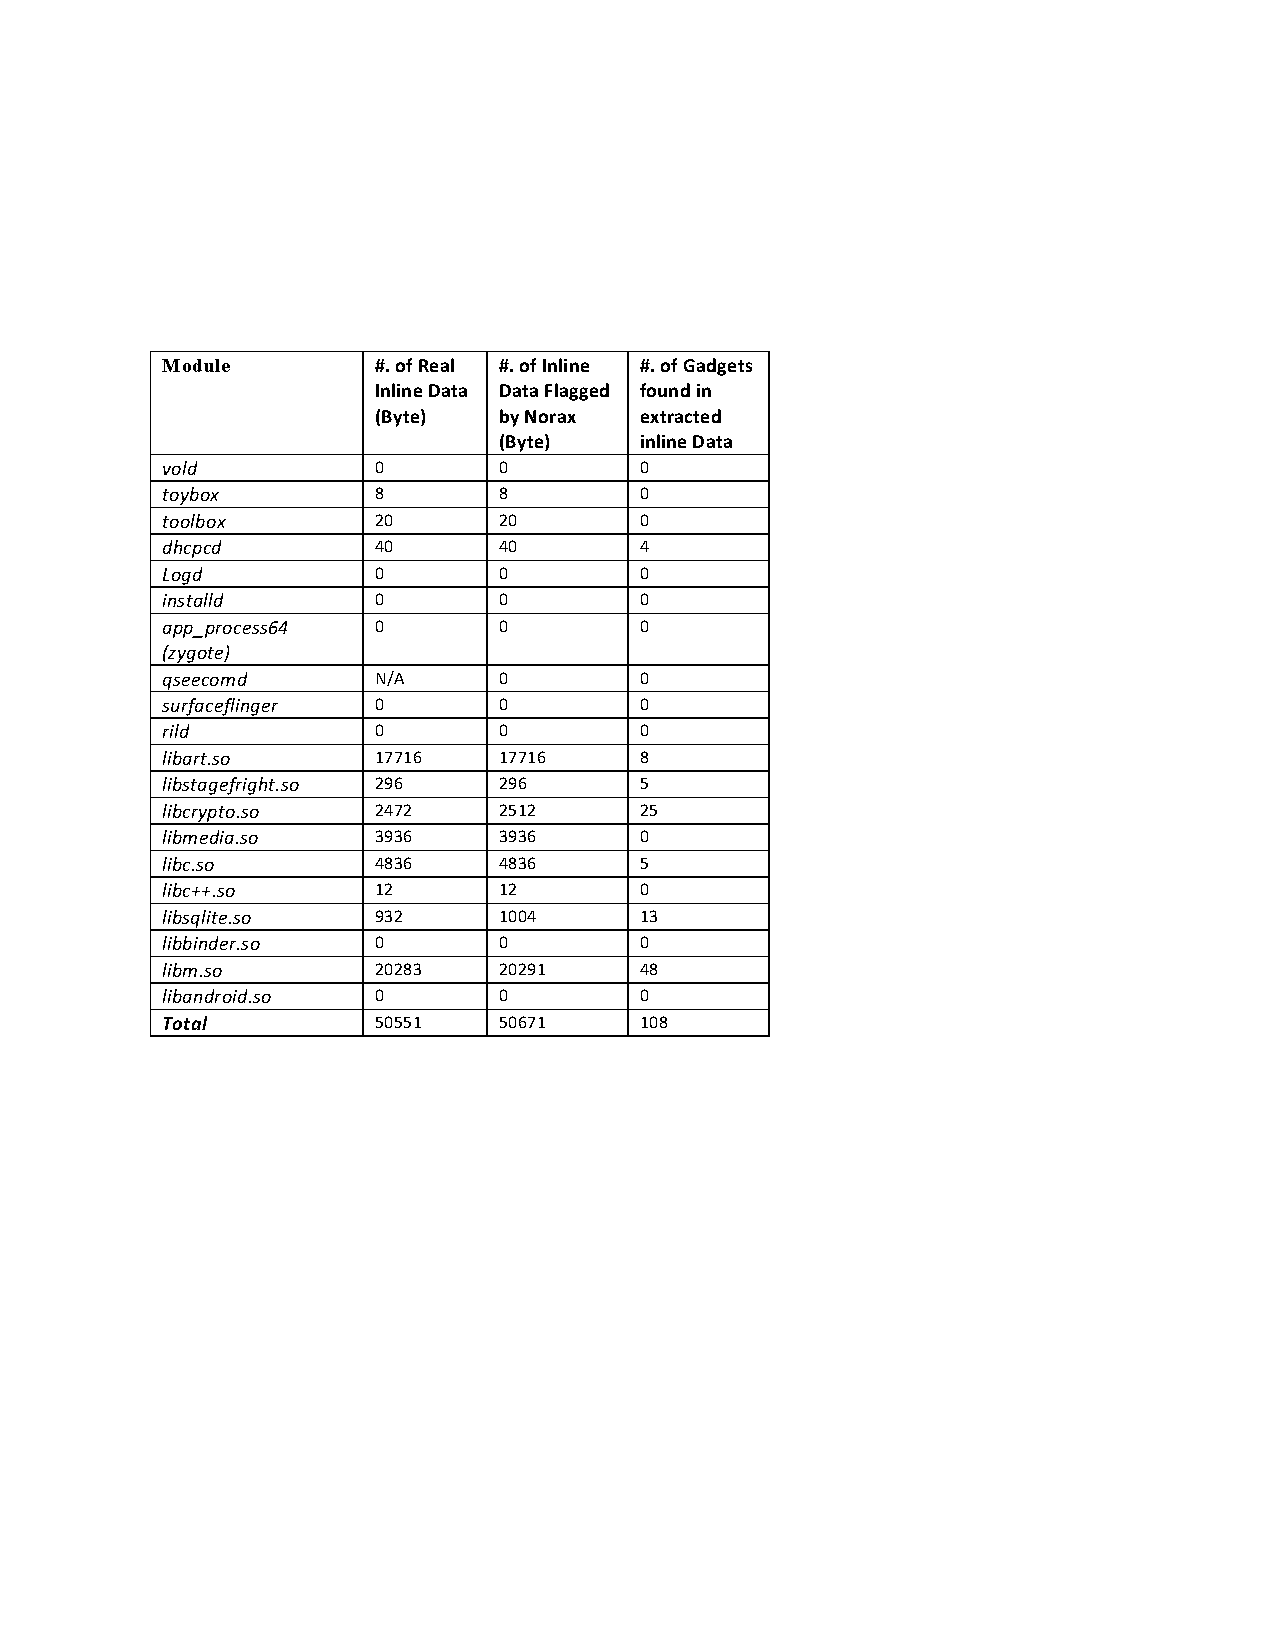
\includegraphics[scale=0.76]{norax/figures/rewrite-effect-sec}
	\end{minipage}
\end{table*}



%\begin{table}[h]
%\caption{Binary transformation correctness test.}
%\label{tab:eval-rewrite}
%\begin{center}
%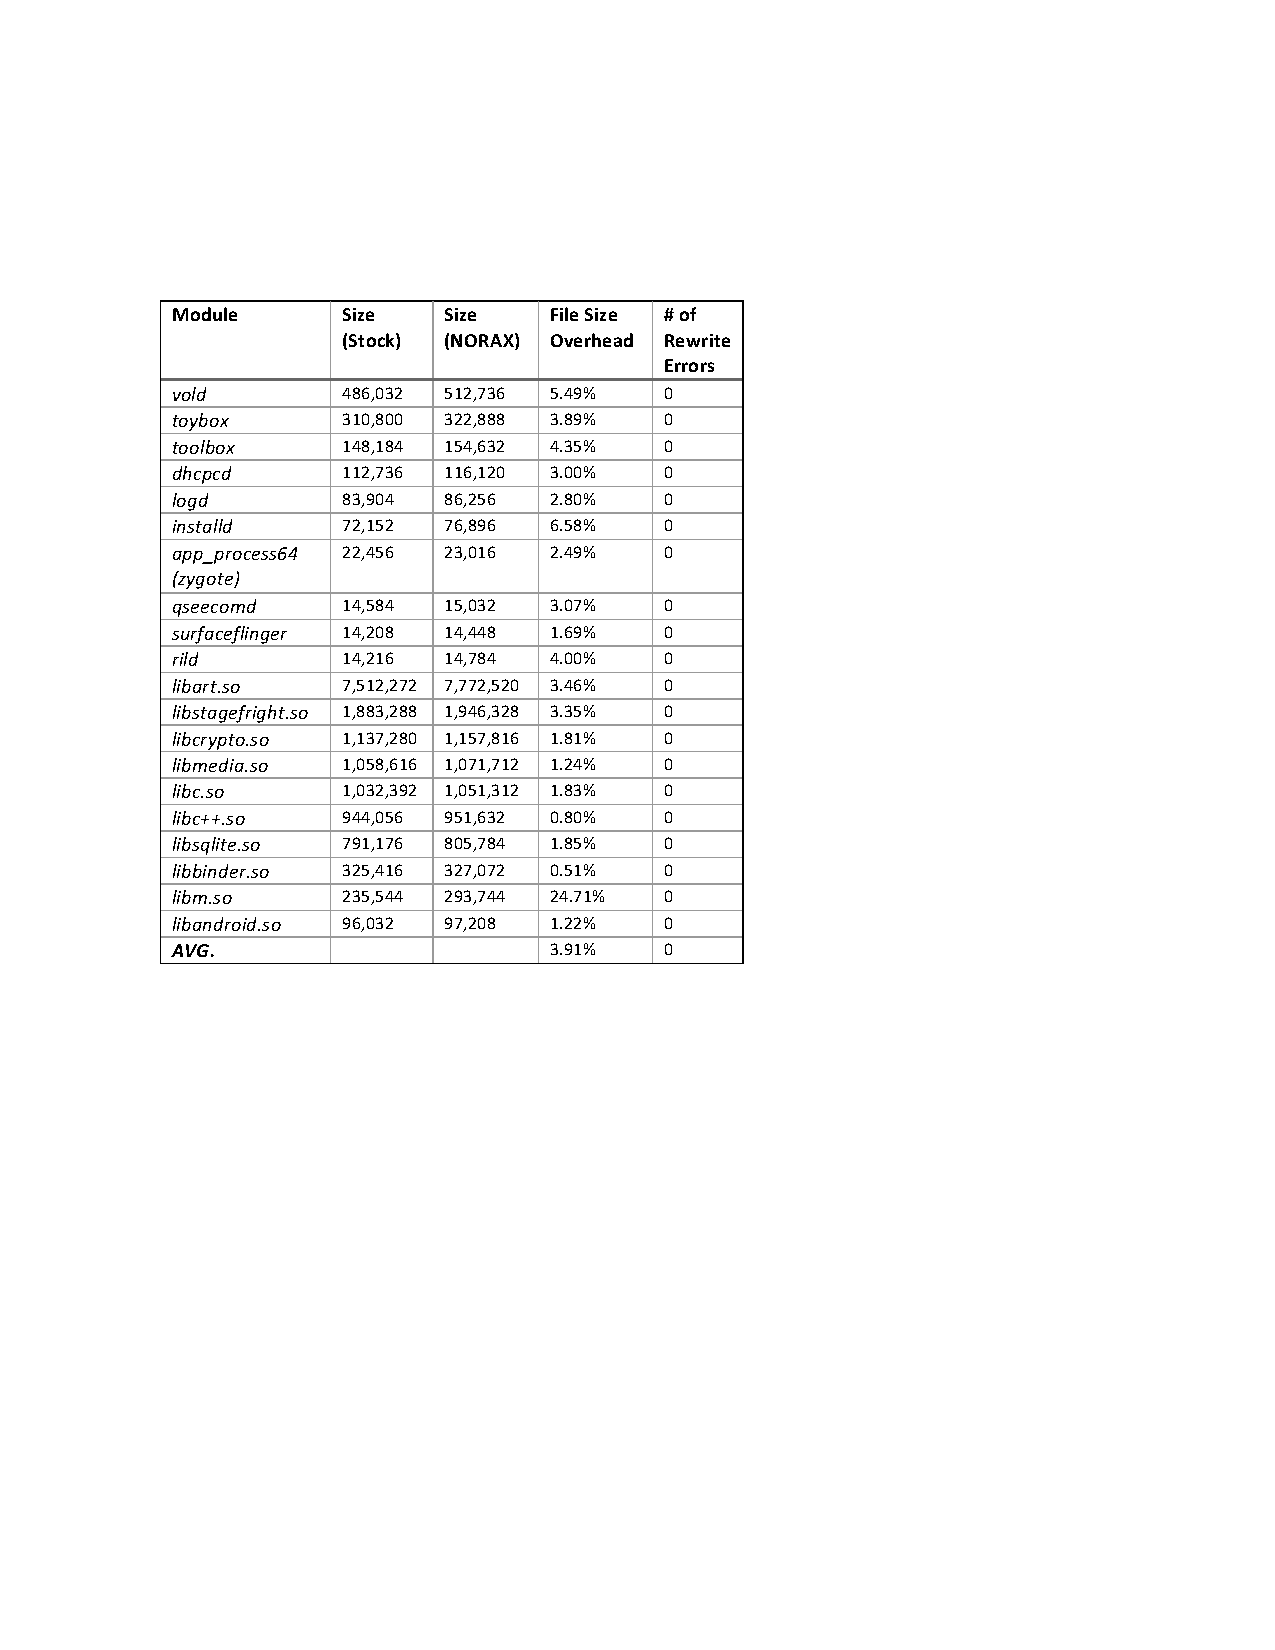
\includegraphics[scale=0.80]{norax/figures/rewrite-correctness}
%\end{center}
%\end{table}
%
%%--analysis correctness: how many code are misflagged as data by us
%%--also security impact that the code misflagged by us are readable and executable to attackers
%\begin{table}[ht]
%\begin{center}
%\caption{Embedded data identification correctness, empirical experiment
%shows our analysis works well in AArch64 COTS ELFs, with {\bf zero} false negative rate and very low false positive rate in terms of finding embedded data. The last column shows the negligible number of leftover gadgets in the duplicated embedded data set.}
%\label{tab:embedgadgets}
%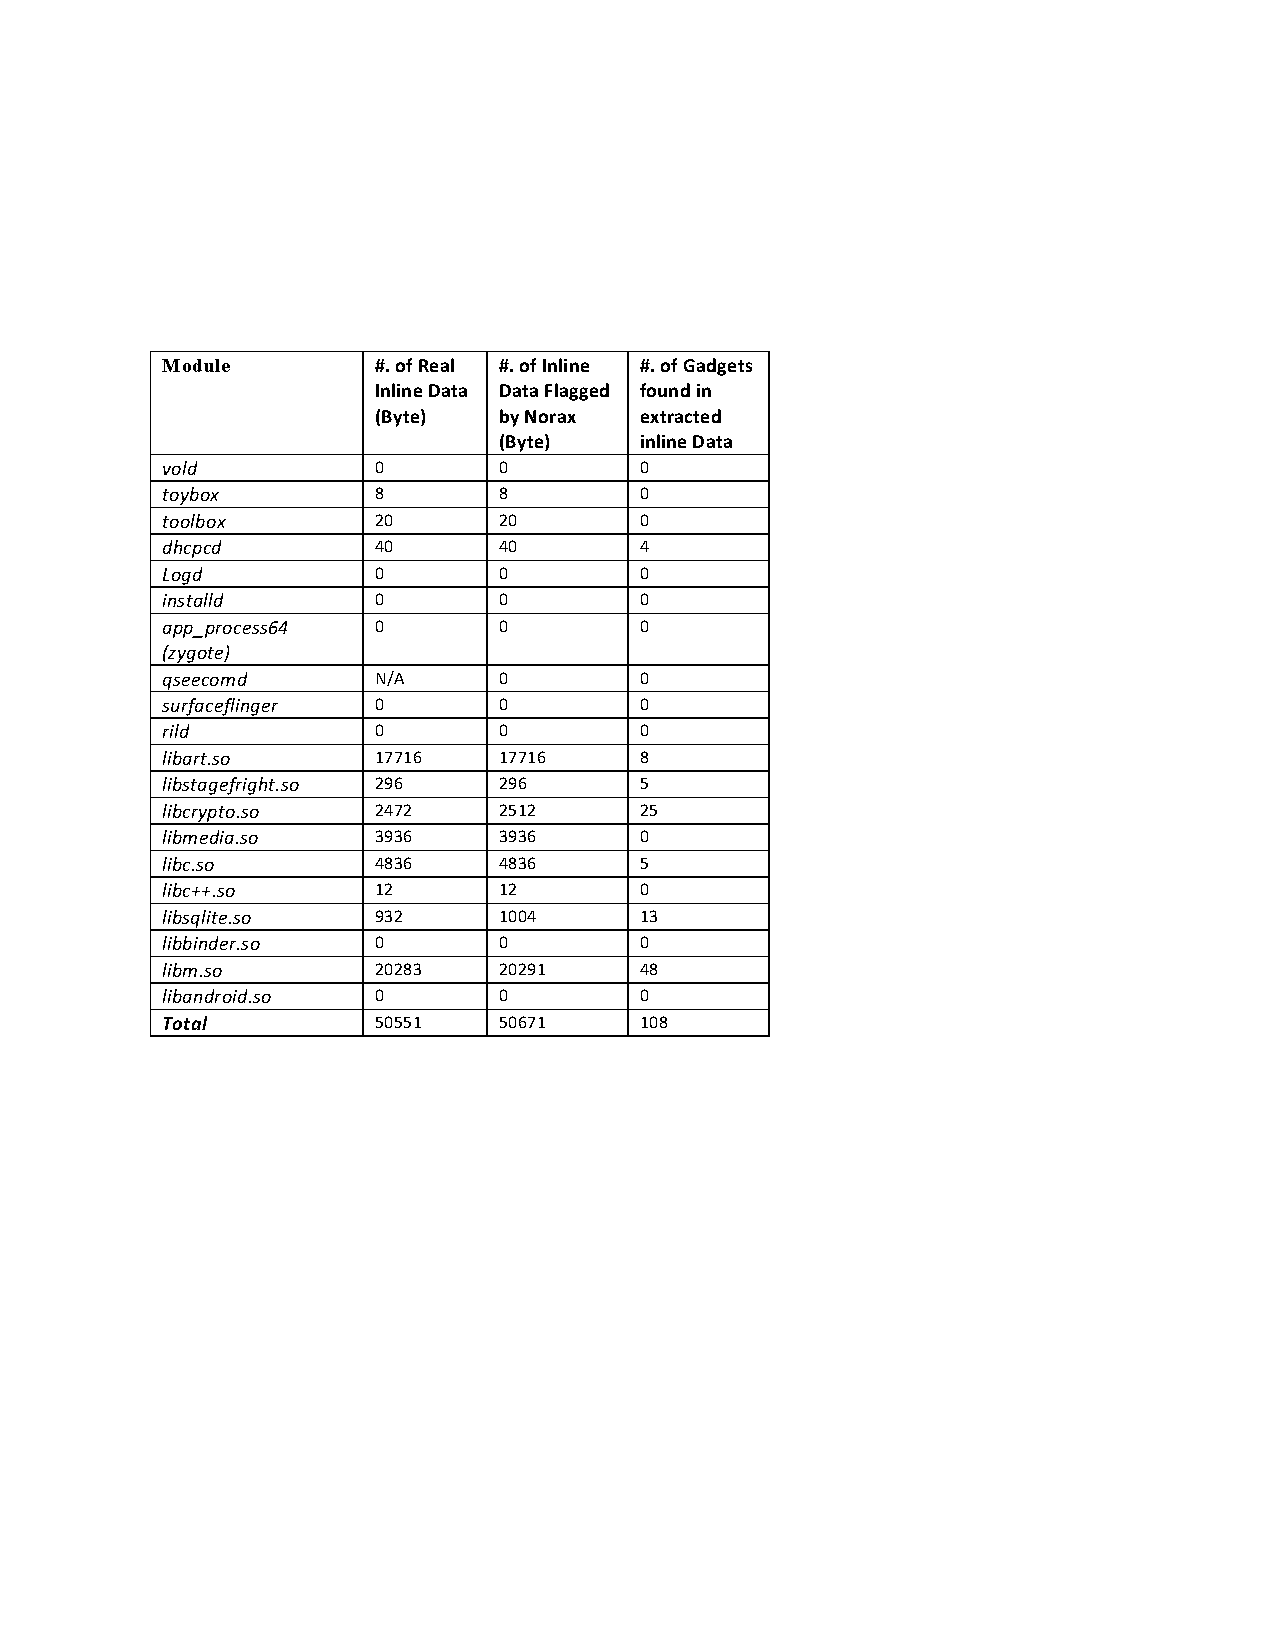
\includegraphics[scale=0.76]{norax/figures/rewrite-effect-sec}
%\end{center}
%\end{table}

%\subsubsection{Overheads and Security Impact}

\point{Size Overhead}
In our functionality test, the sizes of our selected binaries range from $\approx$14K to $\approx$7M,
as shown in Table~\ref{tab:eval-rewrite}. After transformation, the
binary sizes increased by an average of 3.91\%.  Note that $libm.so$
is a outlier, as its file size increased much more
than others. After manual inspection, we found that this math library has a lot of constant values
hardcoded in various mathematical functions such as $casinh()$,
$cacos()$. As an optimization,  the compiler embeds this large set of constant data into the code section to
fully exploit spatial locality, which translates to more metadata generated by \NORAX during the patching stage. 


\point{Performance Overhead}
%todo:try to use a more advance read-write lock to see if we can bring the execl runtime overhead down to single digit
We used Unixbench\cite{unixbench} to measure the performance of our system. 
The benchmark consists of two types of testing programs: (\rom{1}) User-level CPU-bound programs; (\rom{2}) System benchmark programs that evaluate I/O, process creation, and system calls, etc. We ran the benchmark on both the stock and patched binaries, repeating three times in each round. We then derived the average runtime and space overhead, which are given in Figure~\ref{fig:unixbench}.

For the runtime overhead, the average slowdown introduced by \NORAX is 1.18\%. The overhead mainly comes from the system benchmark programs, among which $Execl$ shows the maximum slowdown. Investigating its source code, we found that this benchmark program keeps invoking the \emph{exec} system call from the same process to execute itself over and over again, thus causing \NLoader to repeatedly prepare new book-keeping structures and destroy old ones (\S~\ref{subsec:loader}). This process, in turn, leads to multiple locking and unlocking operations, hence the relatively higher overhead. Fortunately, we do not find this behavior common in normal programs. In addition, some simple optimizations are possible: (\rom{1}) employing a more fine-grained locking mechanism; (\rom{2}) reusing the book-keeping structures when \emph{exec} loads the same image.

%For space overhead, on average \NORAX introduces 1.78\% increase in maximum resident memory and 3.90\% increase in file sizes. Table~\ref{tab:eval-rewrite} shows the file size increase for individual programs.  Both resutls indicate negligible space overhead for \NORAX system. The space overhead is proportionate to the amount of embedded data as well as their references. On the other hand, the \NORAX header incurs a fixed amount of space overhead. If not much embedded data exist, the references and the header become the major contributor to the space overhead.
   
\begin{figure}[h]
\begin{center}
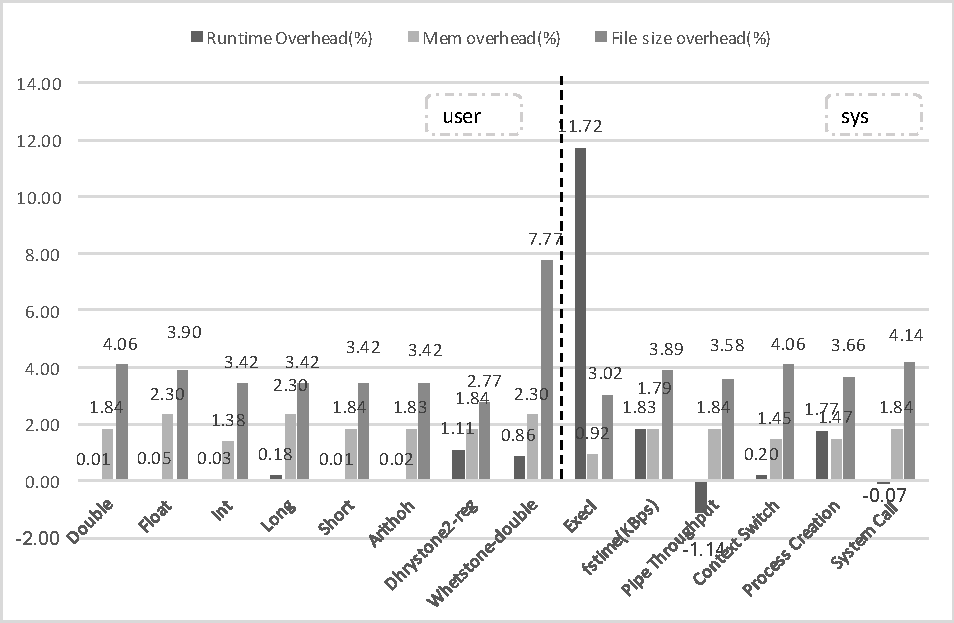
\includegraphics[scale=0.52]{norax/figures/unixbench}
\caption{Unixbench performance overhead for unixbench binaries, including runtime, peak resident memory and file size overhead (left: user tests, right: system tests) }
\label{fig:unixbench}
\end{center}
\end{figure}

\point{Security Impact}
Since \norax duplicates the \emph{embedded data} in code sections, they are in theory still reusable by adversaries. we conduct a gadget searching experiment in the duplicated \emph{embedded data} appended at the end of the converted binaries. Table~\ref{tab:embedgadgets} shows the number of available gadgets we found in those data. As the result shows, available gadgets are actually very rare even in the binaries that have a lot of \emph{embedded data} such as $libm.so$, we believe this is because the majority of those duplicated bytes are by themselves not decodable. Also note that the shown numbers are upper bounds of the available gadgets. Because, in the executable code section, where the original \emph{embedded data} reside, the bytes that form the gadgets may not be placed next to each other.

